\section{Medical Case Assignment}

Complex assignments inevitably vary across courses. As a first step toward
studying how to automate grading of such assignments, we  use a medical
case assignment in the veterinary medicine domain for our study. At a high
level, such an assignment represents a typical type of analysis assignment
where the students are given a case description with both an unstructured
text description as well as some structured data (e.g., lab test results),
and are asked to perform an analysis of the case. The analysis generally
involves 1) selecting relevant content from the case description, which can
be selected from both the text part and the structured data, 2) answering
questions with short textual answers, and 3) writing assessments in
natural language text.

More specifically, the case exercises were developed using
the WhenKnowingMatters (WKM) web-based case formulation
software\footnote{\url{http://www.whenknowingmatters.com}} which
facilitates development and exchange of text-based cases while allowing
students to objectify their observations from a case and manipulate them in
an outline format around a suggested scaffold provided by the instructor.
The student's analysis is then rendered into a structured text format to
facilitate automatic grading.

\begin{figure*}[ht]
\begin{centering}
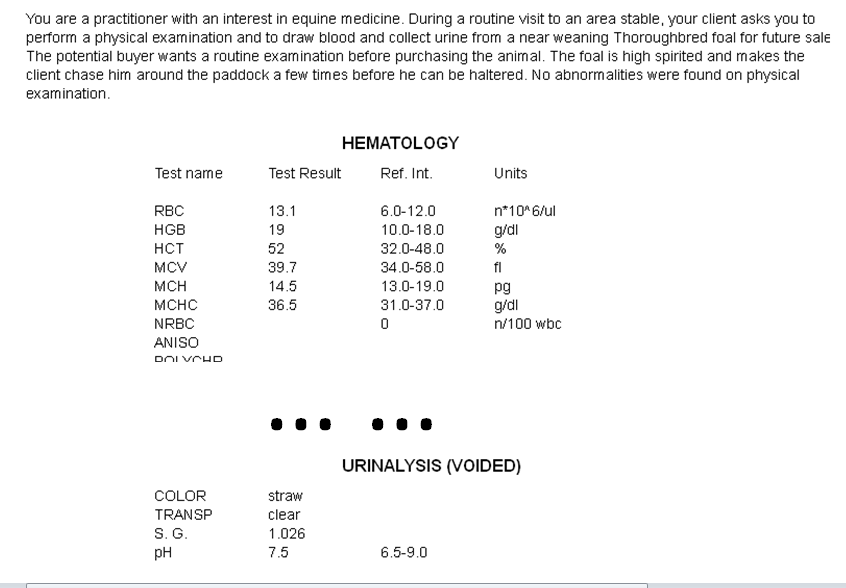
\includegraphics[scale=0.45]{case-desc-small.png}
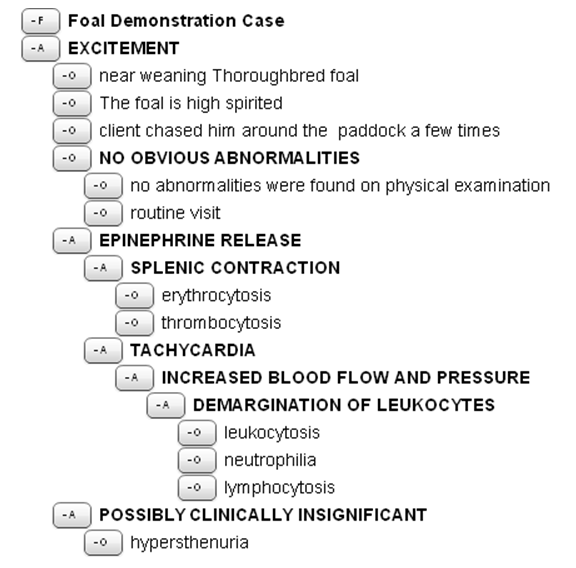
\includegraphics[scale=0.55]{student-work-small.png}
\end{centering}
\caption{An example of case description (left) and student assessment (right)}
\label{fig:example}
\end{figure*}

Due to the lack of automated grading tools, the assignments are currently
graded manually. An assessment rubric designed prior to instruction was
used by the instructor to evaluate student performance on a subjective,
5-point scale (listed here in increasing order): novice, beginner,
competent, proficient, and expert. Rubric categories were related to
elements of critical thinking and communication:
\begin{enumerate}
\item {\bf Questions:} Developing relevant refining (or clarifying)
 questions to answer based upon an honest assessment of current knowledge
 base.
\item {\bf Answers:} Approach to seeking answers to developed
 questions; literature search, etc.
\item {\bf Quality:} Judgment of quality of information; awareness and
 application of standards of a discipline, bias detection including
 appropriate humility to detect one’s own potential bias, application of
 statistical concepts.
\item {\bf Analysis:} Analysis of an argument.
\item  {\bf Clarity:} Clarity and communication of thought; conciseness,
 grammar, spelling, elocution.
\item {\bf Application:} Application and understanding of appropriate
 disciplinary content.
\end{enumerate}


\begin{table}
    \begin{centering}
        \begin{tabular}{l|c}
            analysis & 2.6355 $\pm$ 0.7660
            \\\hline
            answers & 3.0280 $\pm$ 0.7668
            \\\hline
            application & 2.8692 $\pm$ 0.5651
            \\\hline
            clarity & 3.3832 $\pm$ 0.9437
            \\\hline
            quality & 3.1121 $\pm$ 0.9795
            \\\hline
            questions & 2.8224 $\pm$ 0.6810
        \end{tabular}
        \caption{Mean and standard deviation of ranks in each of the
        rubric dimensions we study.}
        \label{table:grade-stats}
    \end{centering}
\end{table}


For our experiments, we used a data set consisting of $n = 107$ student submissions for one medical case
analysis assignment in a veterinary medicine course at XXXX institution.
Each was graded according to the rubric detailed above.  We report the mean
rank and standard deviation for each of these six labels in
Table~\ref{table:grade-stats}; where 1 corresponds to novice and 5 to
expert. The instructor also created a ``gold standard'' assessment for the
assignment case, which is available for the automated grading tool to use.
We wish we could use a much larger data set, but the size of the data set is limited
by the amount of manual work needed for grading, which is precisely our motivation for
studying how to automate grading.  

Figure~\ref{fig:example} shows an example of a very simple case and a typical
student answer. In the case description, the student can see a text
description of the case and a number of lab test results in the form of
structured data. The student assessment is seen to be a semi-structured
text with indented structures based on a scaffold provided by the
instructor. Multiple tags indicate different kinds of answers, including,
e.g., selected content from the original case description, selected lab
tests (both are ``observations''), and text input by the student reflecting
his/her assessment (called ``analysis'').

Because of the complexity, automated grading of such an assignment is very
challenging. First, due to variations across different assignments, it is
almost impossible to learn from the grading results of one assignment to
automate grading of another (often called ``transfer learning''), even
though such an ``inter-assignment'' automated grading is ideal.  We thus
focus on a more realistic setting of attempting to automate the grading
after the instructor has already graded some assignments, which we may
refer to as ``intra-assignment'' automated grading, which, strictly
speaking, is actually semi-automatic grading.  Our goal is thus to study
whether and how we can leverage machine learning to learn from the graded
assignments to reduce the grading burden on an instructor, either by
directly predicting grades or by providing a ranking as a scaffolding for
assigning grades.
